\documentclass{beamer}
\usetheme{Madrid}
\usepackage[utf8]{inputenc}
\usepackage[T2A]{fontenc}
\usepackage[russian]{babel}
\usepackage{amsmath, amssymb}
\usepackage{graphicx}
\usepackage{csquotes}
\usepackage[style=gost-footnote,
bibstyle=gost-footnote,
language=russian,
backend=biber
]{biblatex}
\addbibresource{bib.bib}

\title{Исследование влияния вида задачи для уравнения гармонического осциллятора на решение PINN}
\author{Донецков А.Д., Бакакин В.Д., Жулев Е.М.\\
\textit{
    Институт Лазерных и плазменных технологий\\
    НИЯУ МИФИ\\
    г. Москва
}}
\date{20 декабря 2024}

\setbeamertemplate{footline}{%
  \leavevmode%
  \hbox{%
    \begin{beamercolorbox}[wd=.33\paperwidth,ht=2.25ex,dp=1ex,center]{author in head/foot}%
      Андрей, Валерий, Егор
    \end{beamercolorbox}%
    \begin{beamercolorbox}[wd=.33\paperwidth,ht=2.25ex,dp=1ex,center]{title in head/foot}%
      PINN для осциллятора
    \end{beamercolorbox}%
    \begin{beamercolorbox}[wd=.33\paperwidth,ht=2.25ex,dp=1ex,center]{date in head/foot}%
      \insertshortdate
    \end{beamercolorbox}%
  }%
  \vskip0pt%
}

\begin{document}

\begin{frame}
    \titlepage
\end{frame}

\begin{frame}{Содержание}
    \tableofcontents
\end{frame}

\section{Введение}
\begin{frame}{Введение}
    \begin{itemize}
        \item Решение уравнений движения гармонического осциллятора важно в вычислительной физике и механике.
        \item Гармонический осциллятор описывается дифференциальными уравнениями второго и первого порядка.
        \item Развитие нейросетевых методов, особенно PINN.~\footcite{Lagaris1998,Raissi2019} позволила более быстро получить приемлимые результаты.
        \item \textbf{Цель}: сравнить влияние различных формулировок задачи Коши на метод PINN.
    \end{itemize}
\end{frame}

\section{Постановка задачи}
\subsection{Система ОДУ второго порядка}
\begin{frame}{ОДУ второго порядка}
    \begin{equation}
    \begin{cases}
    \dfrac{d^2x}{dt^2} + \omega_0^2 x = -A\cos(\omega t), \\
    x(0) = x_0, \\
    \dfrac{dx}{dt}(0) = v_0.
    \end{cases}
    \end{equation}
\end{frame}

\subsection{Системы ОДУ первого порядка}
\begin{frame}{Системы ОДУ первого порядка}
    \begin{minipage}[t]{0.45\textwidth}
        \begin{equation}
            \begin{cases}
            \dfrac{dx}{dt} = y, \\
            \dfrac{dy}{dt} = -\omega_0^2 x - A\cos(\omega t), \\
            x(0) = x_0, \\
            y(0) = v_0.
            \end{cases}
        \end{equation}
        \vspace{0.5cm}
    \end{minipage}
    \begin{minipage}[t]{0.45\textwidth}
        \begin{equation}
            \begin{cases}
            \dfrac{dx}{dt} = \omega_0 y - \dfrac{A}{\omega}\sin(\omega t), \\
            \dfrac{dy}{dt} = -\omega_0 x, \\
            x(0) = x_0, \\
            y(0) = \dfrac{v_0}{\omega_0}.
            \end{cases}
        \end{equation}
    \end{minipage}

    \begin{block}{Замечание}
        Разные системы дифференциальных уравнений первого порядка могут быть полезны в случаях, когда форма упрощает аналитическое или численное решение, в зависимости от характера внешней силы или других факторов.
    \end{block}

\end{frame}

\section{Ключевые особенности PINN}
\begin{frame}{Преимущества PINN}
    \begin{itemize}
        \item PINN включают физические законы непосредственно в процесс обучения, что позволяет получать физически корректные решения.
        \item Использование автоматического дифференцирования для вычисления градиентов позволяет получить большую точность.
        \item Применимость к различным задачам: ОДУ, УЧП и их системы.
        \item PINN позволяет получить данные быстрее численных методов. Особенно для многомерных случаев. Точность не требует слишком мелкого сидения сетки.
    \end{itemize}
\end{frame}

\begin{frame}{Ограничения PINN}
    \begin{itemize}
        \item Трудности с аппроксимацией разрывных функций.
        \item Низкая эффективность при решении жестких и хаотических систем.
        \item Застревание в локальных оптимумах.
        \item Сложности в балансировке компонентов функции потерь.
    \end{itemize}
\end{frame}

\section{Методология}
\begin{frame}{Методология}
    \begin{itemize}
        \item Одинаковая конфигурация нейросети для всех 3 формулировок:
        \begin{itemize}
            \item Вход: время
            \item 5 скрытых слоёв по 20 нейронов
            \item Функция активации: синус
            \item Выход: 1 или 2 нейрона
        \end{itemize}
        \item Функционал потерь: $loss = loss_{interior} + \lambda_{bc} * loss_{boundary}$, где $\lambda_{bc} = 50$
        \item Оптимизатор: Adam с шагом обучения $10^{-3}$
        \item Обучение на интервале $[-5, 15]$ с шагом $0.05$
        \item Параметры задач Коши:
        \begin{itemize}
            \item $\omega = \omega_F = 2, \frac{F}{m} = 0.25, v_0 = 1$ для резонанса
            \item $\omega = 2, \omega_F = 2.5, \frac{F}{m} = 2, v_0 = 1$ для его отсутствия
        \end{itemize}
    \end{itemize}
\end{frame}

\section{Результаты}
\subsection{ОДУ второго порядка}
\begin{frame}{ОДУ второго порядка}
    \begin{figure}[h!]
        \centering
        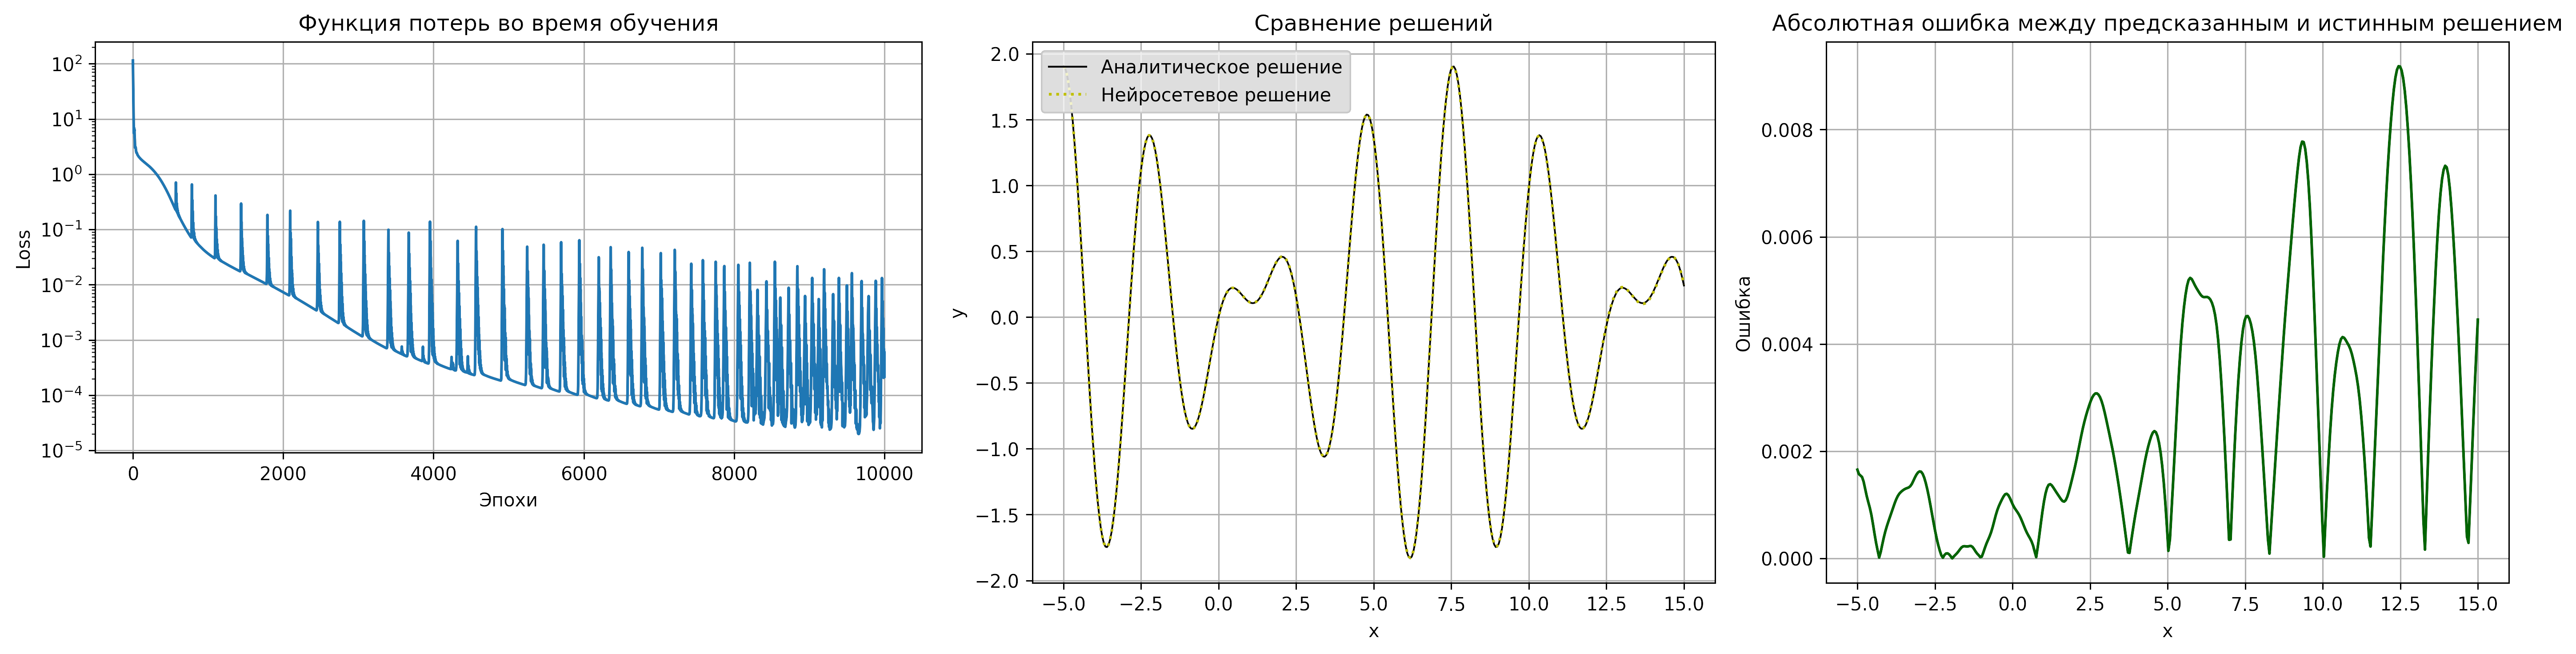
\includegraphics[width=0.9\textwidth]{images/Loss&x_ODE_of_the_second_order.png}
        \caption{Функция потерь для ОДУ второго порядка}
        \label{fig:loss_second_order}
    \end{figure}
    \begin{figure}[h!]
        \centering
        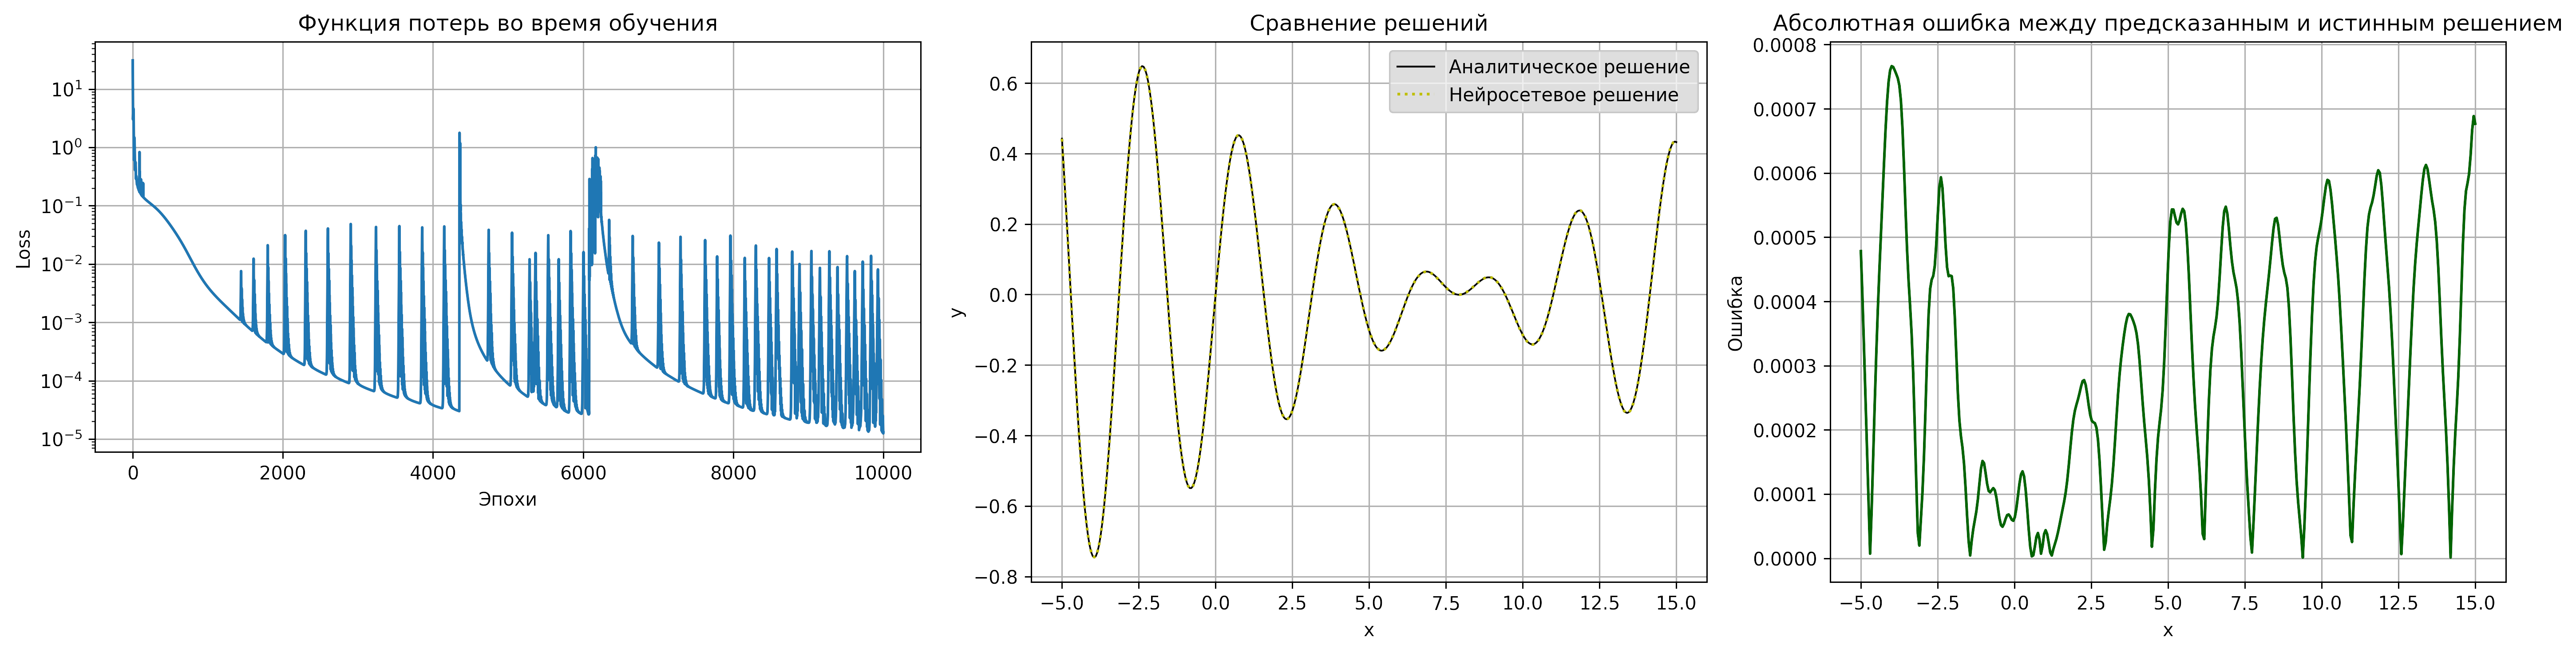
\includegraphics[width=0.9\textwidth]{images/Loss&x_ODE_of_the_second_order_resonance.png}
        \caption{Функция потерь для ОДУ второго порядка с резонансом}
        \label{fig:loss_second_order_resonance}
    \end{figure}
\end{frame}

\begin{frame}{ОДУ второго порядка}
    \begin{table}[h!]
        \centering
        \begin{tabular}{|c|c|c|c|}
        \hline
        \multicolumn{2}{|c|}{\textbf{Без резонанса}} & \multicolumn{2}{|c|}{\textbf{С резонансом}} \\
        \hline
        \textbf{MAE $x, 10^{-2}$} & \textbf{MAE $\dfrac{dx}{dt}, 10^{-2}$} & \textbf{MAE $x, 10^{-2}$} & \textbf{MAE $\dfrac{dx}{dt}, 10^{-2}$} \\
        \hline
        1.1879 & 2.4357 & 1.1877 & 2.4116 \\
        1.2033 & 2.4247 & 1.2502 & 2.5555 \\
        1.6343 & 3.0803 & 1.4000 & 2.8247 \\
        1.2127 & 2.4514 & 1.2128 & 2.4863 \\
        1.1406 & 2.3287 & 1.2032 & 2.3616 \\
        \hline
        \textbf{1.2758} & \textbf{2.5442} & \textbf{1.2508} & \textbf{2.5279} \\
        \hline
        \end{tabular}
        \caption{ОДУ второго порядка}
    \end{table}

    \begin{itemize}
        \item Высокая точность и быстрая сходимость.
        \item Возможные проблемы с локальными минимумами.
    \end{itemize}

    \begin{alertblock}{Заметим:}
        MAE $x$ в 2 раза меньше MAE $\dfrac{dx}{dt}$.
    \end{alertblock}
\end{frame}

\subsection{Система ОДУ первого порядка}
\begin{frame}{Система ОДУ первого порядка}
    \begin{figure}[h!]
        \centering
        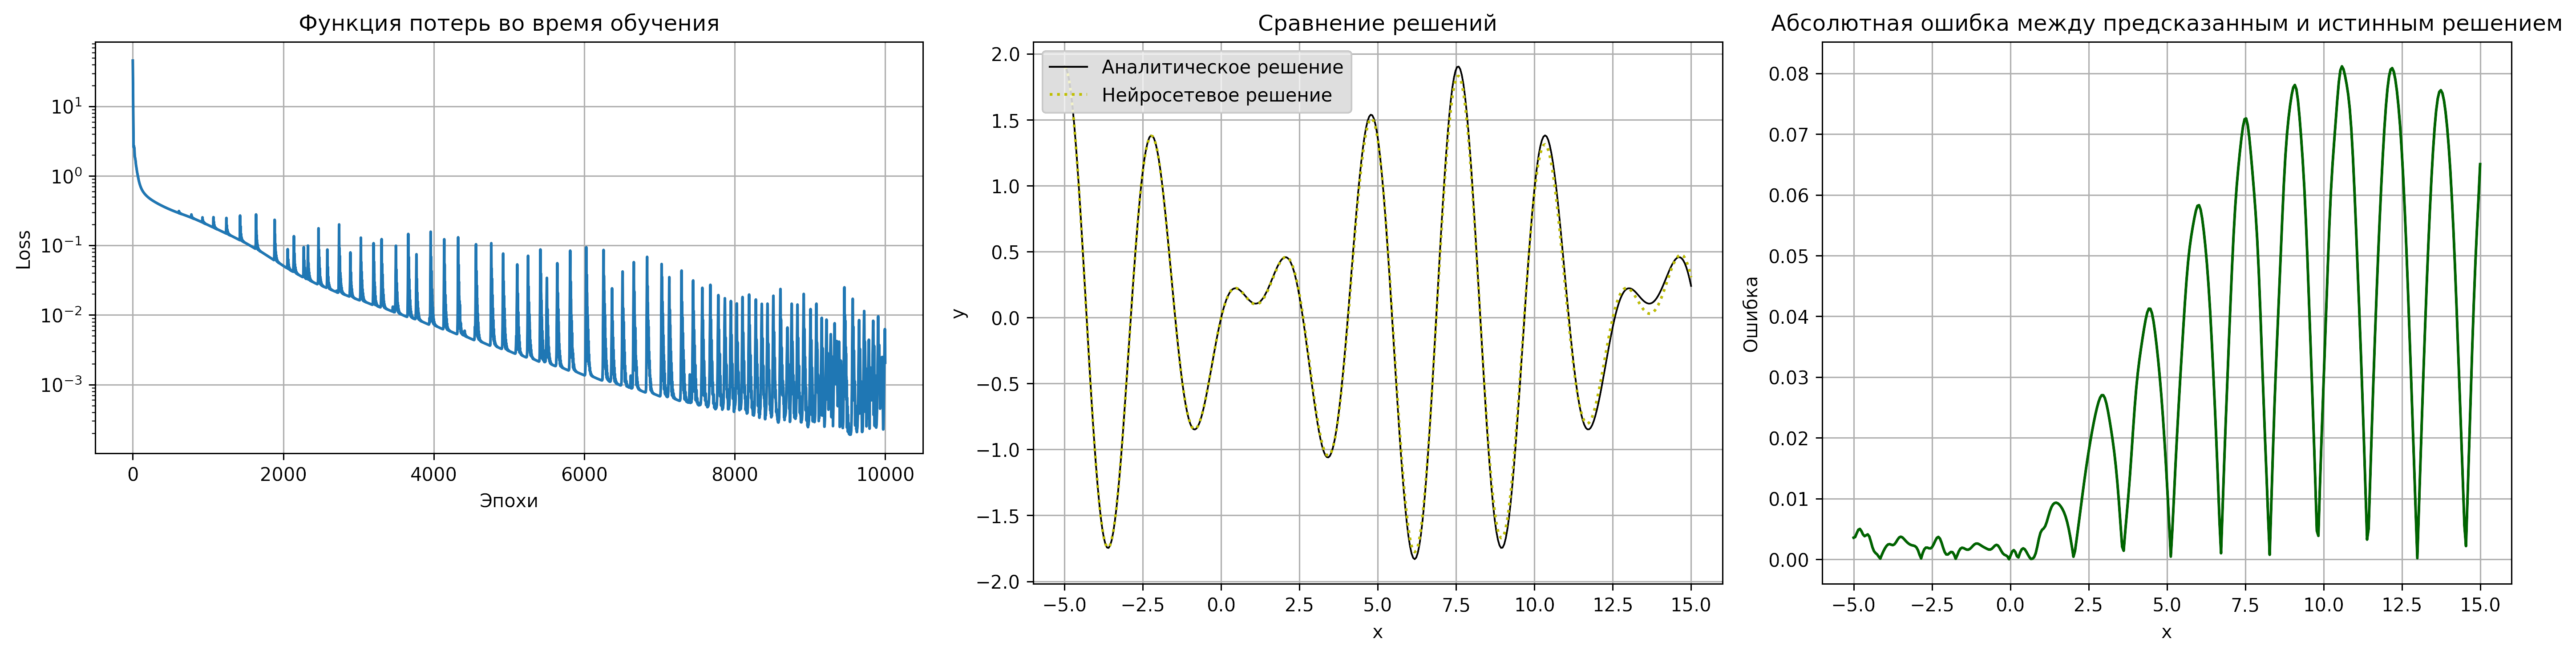
\includegraphics[width=0.9\textwidth]{images/Loss&x_ODE_of_the_first_order.png}
        \caption{Функция потерь для системы ОДУ первого порядка}
        \label{fig:loss_first_order}
    \end{figure}
    \begin{figure}[h!]
        \centering
        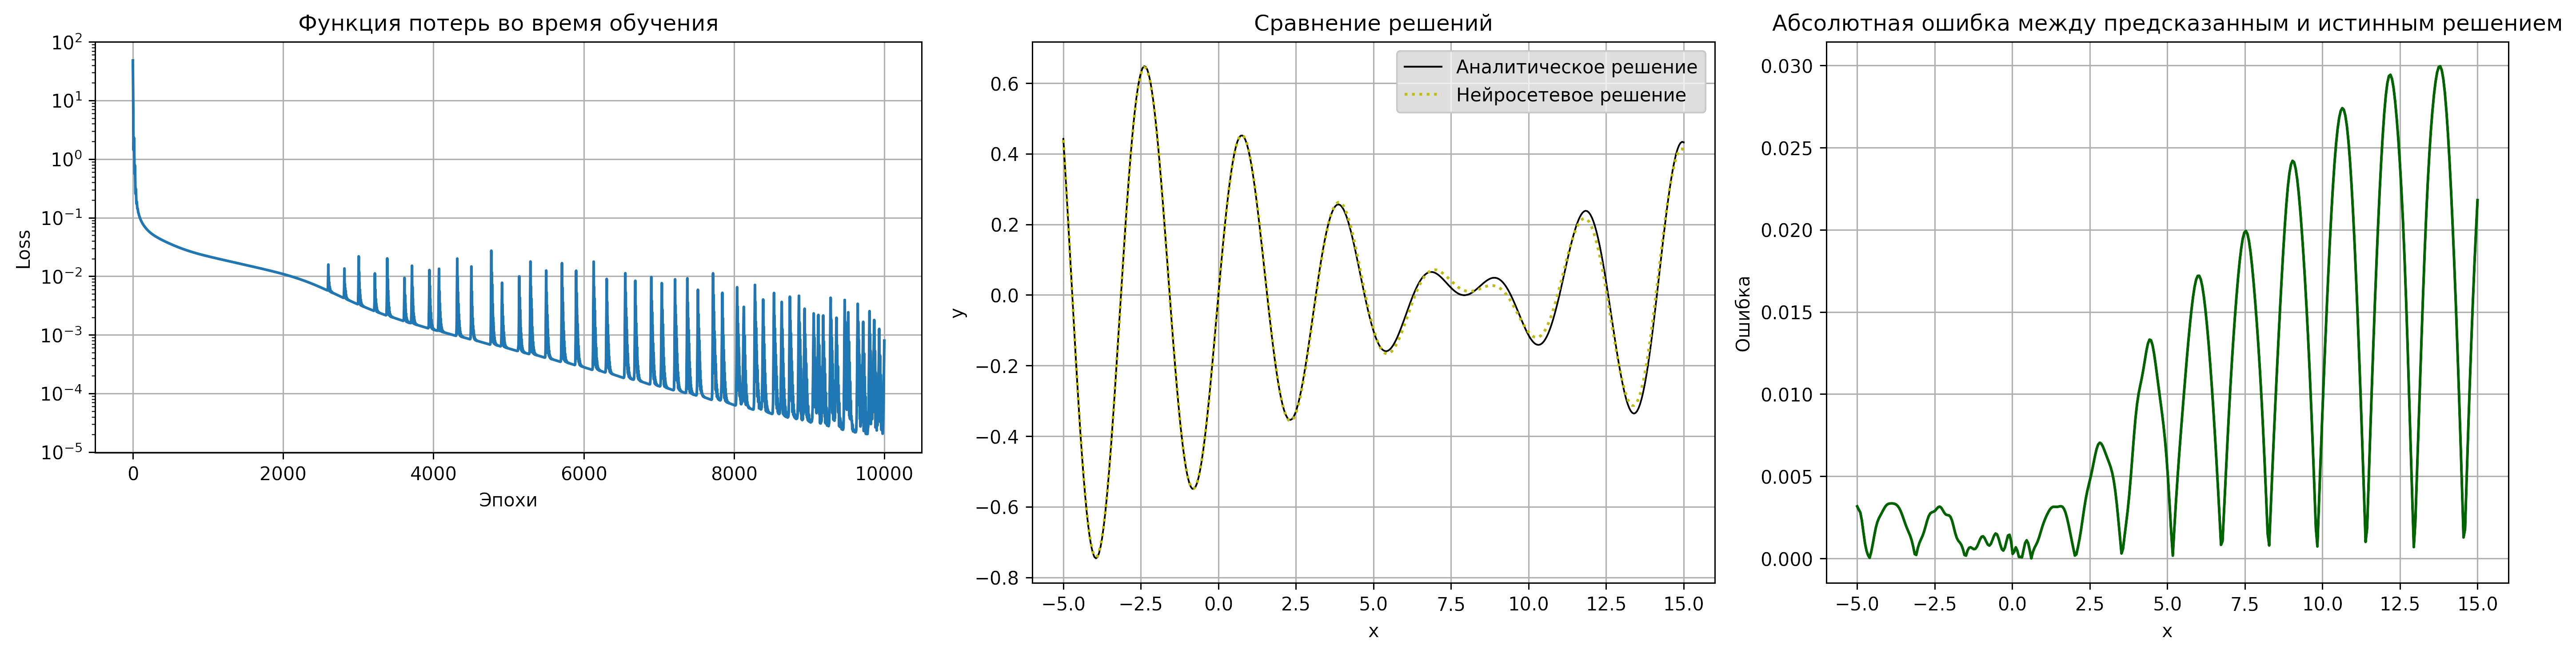
\includegraphics[width=0.9\textwidth]{images/Loss&x_ODE_of_the_first_order_resonance.png}
        \caption{Функция потерь для системы ОДУ первого порядка с резонансом}
        \label{fig:loss_first_order_resonance}
    \end{figure}
\end{frame}

\begin{frame}{Система ОДУ первого порядка с резонансом}
    \begin{table}[h!]
        \centering
        \begin{tabular}{|c|c|c|c|}
        \hline
        \multicolumn{2}{|c|}{\textbf{Без резонанса}} & \multicolumn{2}{|c|}{\textbf{С резонансом}} \\
        \hline
        \textbf{MAE $x, 10^{-2}$} & \textbf{MAE $\dfrac{dx}{dt}, 10^{-2}$} & \textbf{MAE $x, 10^{-2}$} & \textbf{MAE $\dfrac{dx}{dt}, 10^{-2}$} \\
        \hline
        4.8092 & 9.8869 & 0.43286 & 0.8909 \\
        3.5429 & 7.2853 & 0.32455 & 0.6793 \\
        3.6680 & 7.4666 & 0.96157 & 1.9562 \\
        3.6264 & 7.4309 & 0.64427 & 1.3446 \\
        2.5681 & 5.4567 & 0.32558 & 0.6419 \\
        \hline
        \textbf{3.6429} & \textbf{7.5053} & \textbf{0.5378} & \textbf{1.1026} \\
        \hline
        \end{tabular}
        \caption{ОДУ первого порядка}
    \end{table}

    \begin{itemize}
        \item Более стабильный, но медленный процесс обучения.
        \item Без резонанса среднее MAE больше ОДУ второго порядка в 3 раза.
        \item Лучшая ОДУ для резонанса.
    \end{itemize}

\end{frame}

\subsection{Альтернативная система ОДУ первого порядка}
\begin{frame}{Альтернативная система ОДУ первого порядка}
    \begin{figure}[h!]
        \centering
        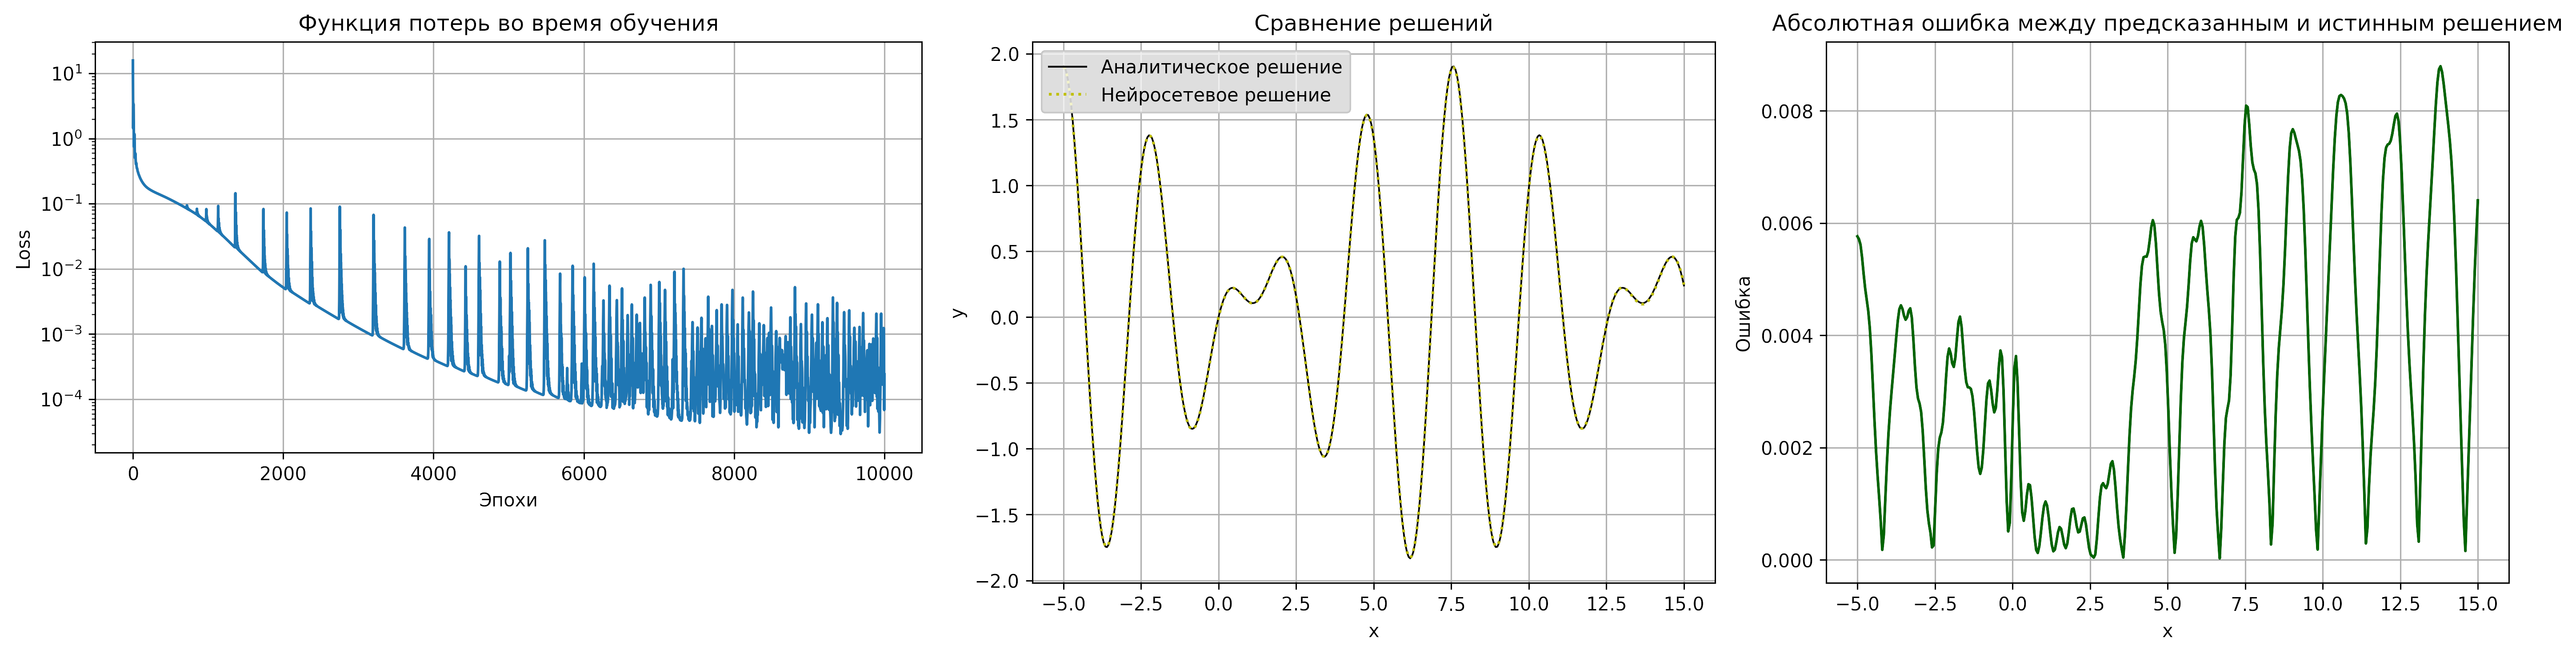
\includegraphics[width=0.9\textwidth]{images/Loss&x_alt_ODE.png}
        \caption{Функция потерь для альтернативной системы ОДУ}
        \label{fig:loss_alt}
    \end{figure}
    \begin{figure}[h!]
        \centering
        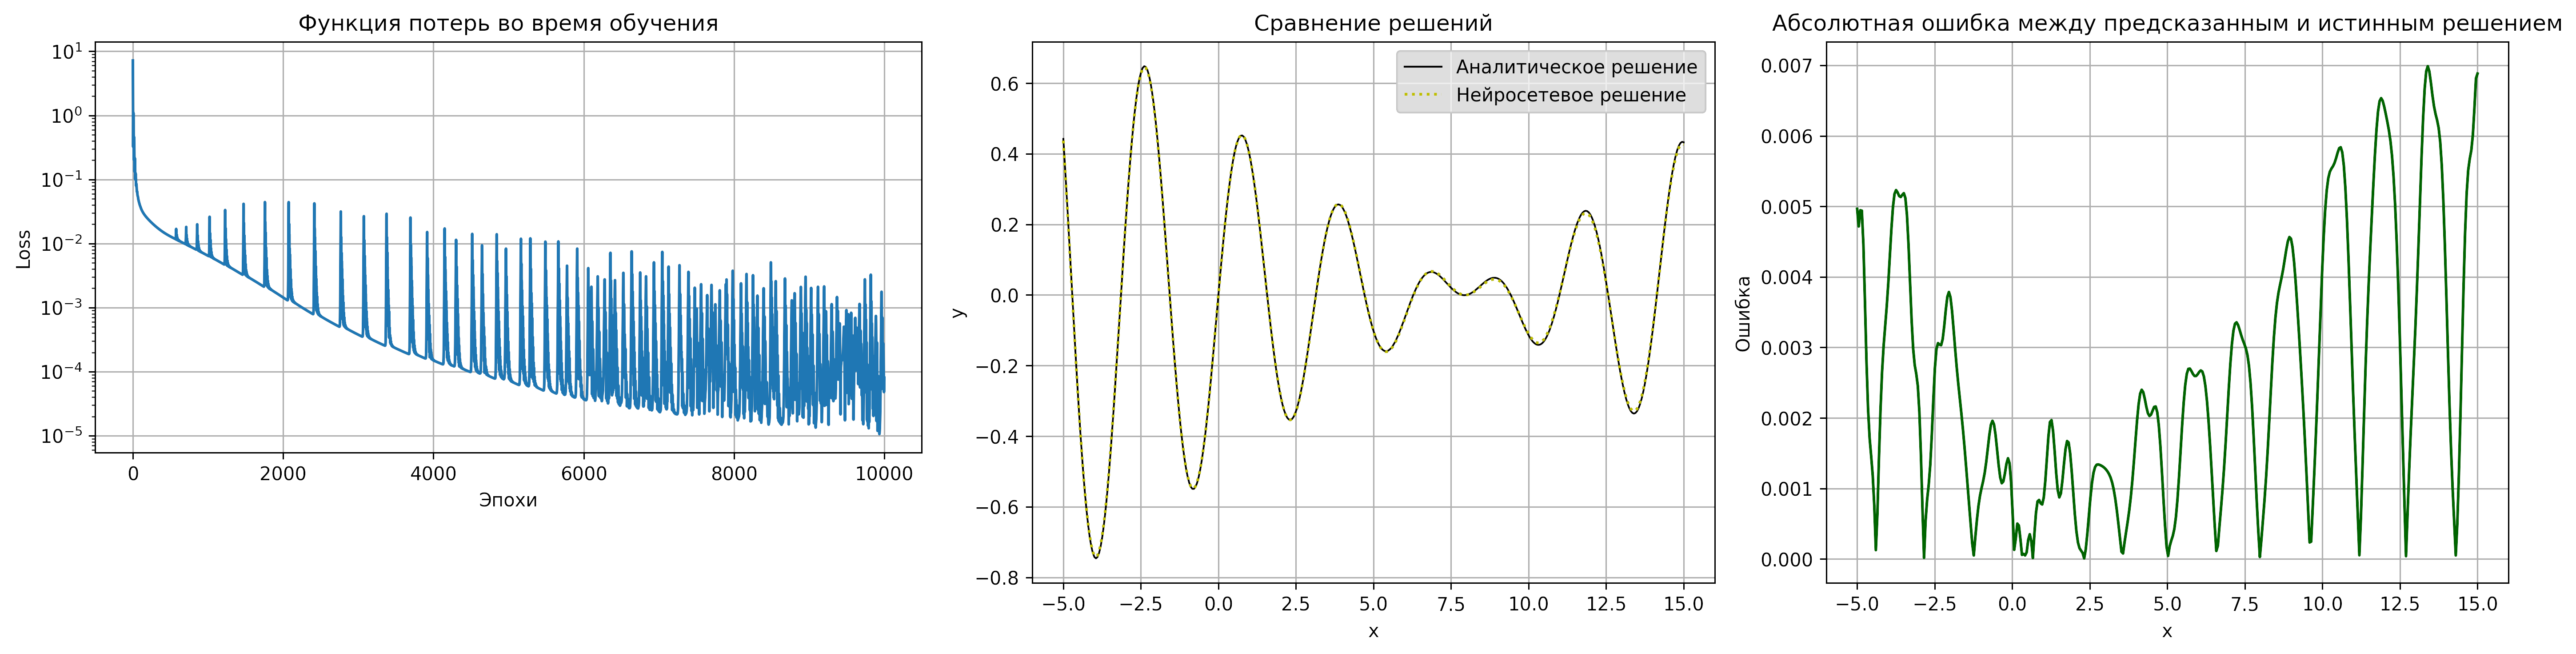
\includegraphics[width=0.9\textwidth]{images/Loss&x_alt_ODE_resonance.png}
        \caption{Функция потерь для альтернативной системы ОДУ с резонансом}
        \label{fig:loss_alt_resonance}
    \end{figure}
\end{frame}

\begin{frame}{Альтернативная система ОДУ первого порядка с резонансом}
    \begin{table}[h!]
        \centering
        \begin{tabular}{|c|c|c|c|}
        \hline
        \multicolumn{2}{|c|}{\textbf{Без резонанса}} & \multicolumn{2}{|c|}{\textbf{С резонансом}} \\
        \hline
        \textbf{MAE $x, 10^{-2}$} & \textbf{MAE $\dfrac{dx}{dt}, 10^{-2}$} & \textbf{MAE $x, 10^{-2}$} & \textbf{MAE $\dfrac{dx}{dt}, 10^{-2}$} \\
        \hline
        1.0991 & 2,3144 & 1.0198 & 2.2316 \\
        2.4914 & 5,1818 & 0.2385 & 0.5340 \\
        1.0468 & 2,2011 & 1.2542 & 2.6190 \\
        0.4407 & 0,9656 & 1.3087 & 2.7650 \\
        0.9234 & 1,9852 & 0.2077 & 0.4756 \\
        \hline
        \textbf{1.2003} & \textbf{2.5296} & \textbf{0.8058} & \textbf{1.7250} \\
        \hline
        \end{tabular}
        \caption{Альт. ОДУ первого порядка}
    \end{table}

    \begin{itemize}
        \item Большая точность по сравнению с первой системой.
        \item Менее стабильный процесс обучения.
        \item Достигается точность, близкая к ОДУ второго порядка.
    \end{itemize}
\end{frame}

\section{Выводы}
\begin{frame}{Выводы}
    \begin{itemize}
        \item Выбор постановки задачи Коши существенно влияет на эффективность и точность PINN.
        \item \textbf{ОДУ второго порядка:}
        \begin{itemize}
            \item Быстрая сходимость.
            \item Возможны локальные минимумы.
        \end{itemize}
        \item \textbf{Системы ОДУ первого порядка:}
        \begin{itemize}
            \item Повышенная устойчивость обучения.
            \item Снижение точности и увеличение времени сходимости.
        \end{itemize}
        \item \textbf{Альтернативная система ОДУ первого порядка:}
        \begin{itemize}
            \item Высокая точность.
            \item Более стабильный процесс оптимизации.
        \end{itemize}
    \end{itemize}
    Мы приглашаем заинтересованных исследователей использовать и развивать представленный подход.~\footfullcite{git}
\end{frame}

\printbibliography

\end{document}